% Visual

\begin{figure}[h]
	\centering
	\begin{minipage}{.5\textwidth}
		\capstart
		\centering
		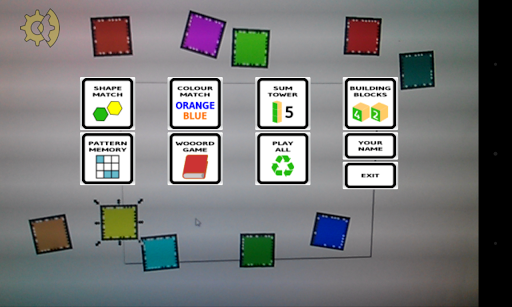
\includegraphics[width=0.9\textwidth]{images/main_menu.png}
		\vspace{-10pt}
		\caption{Screenshot of the main menu.}
		\label{fig:main_menu}
	\end{minipage}%
	\begin{minipage}{.5\textwidth}
		\capstart
		\centering
		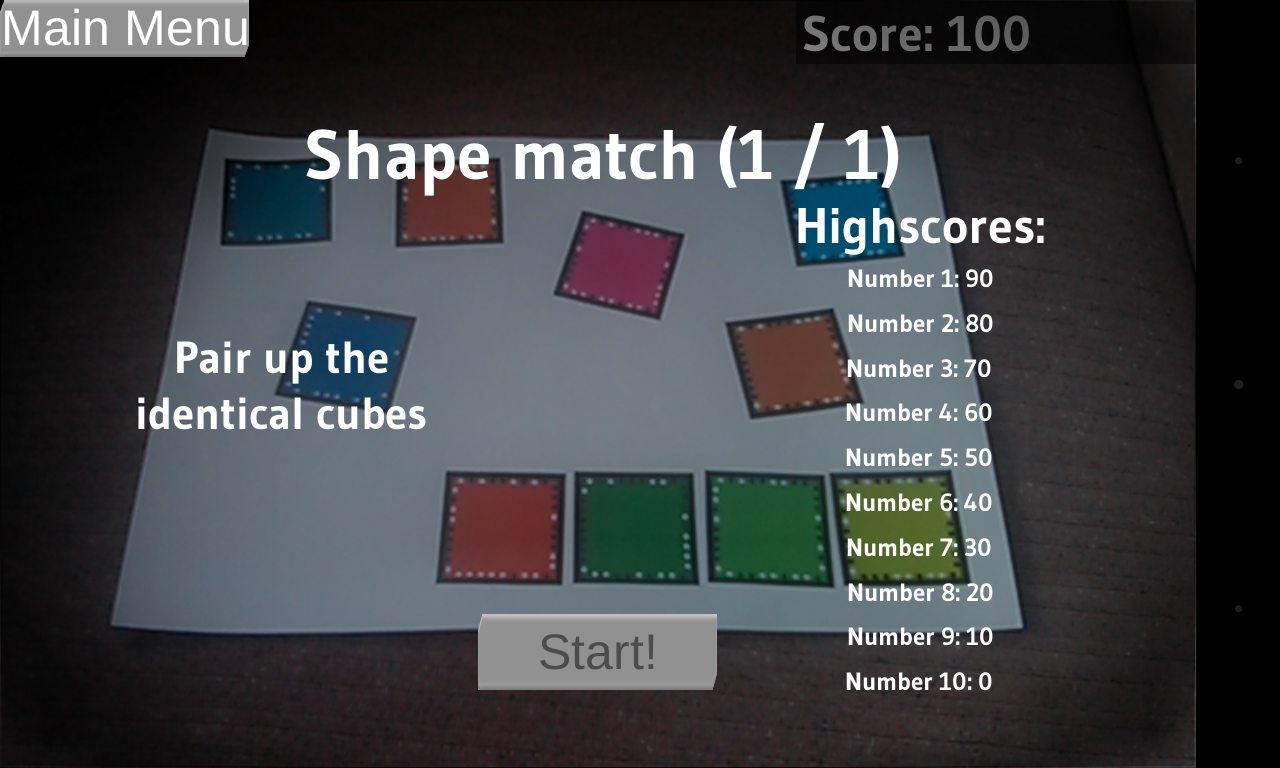
\includegraphics[width=0.9\textwidth]{images/loading_screen.png}
		\vspace{-10pt}
		\caption{Screenshot of a loading screen.}
		\label{fig:loading_screen}
	\end{minipage}%
\end{figure}

\paragraph{}
The main menu cosists of buttons that leads to each the minigames with each button having both the name of the corresponding
minigame and a small illulstration that gives the user a hint to what the user will do.
There is also the "YOUR NAME" and "EXIT" buttons. The "YOUR NAME" button will take the user to a new screen with a input field 
for chaning or setting their username whilst the "EXIT" button will exit the application.
The background behind the buttons is what the devices camera is currently seeing.

\paragraph{}
The second picture shows one of our loading screens, in this case it is the loading screen for {\todo{Legg inn ref til shape match her}}\ref{game:shape_match}.
The loading screens are comprised of two main elements and three smaller elements.
The main elements are the highscore list to the right and a description on the left.
These will introduce the user to what the goal for the minigame is and hopefully encourge the user to do their best everytime to improve the highscore.

The smaller elements are the titlebar that shows the name of the minigame followed by current level of the game and how many levels it has in total.
A button in the top left lets the user return to the main menu and lastly there's the "Start!" button that begins the game.

While in the menu the user can see what the camera is currently seeing in the background behind all these elements.

\begin{figure}[h]
	\centering
	\begin{minipage}{.5\textwidth}
		\capstart
		\centering
		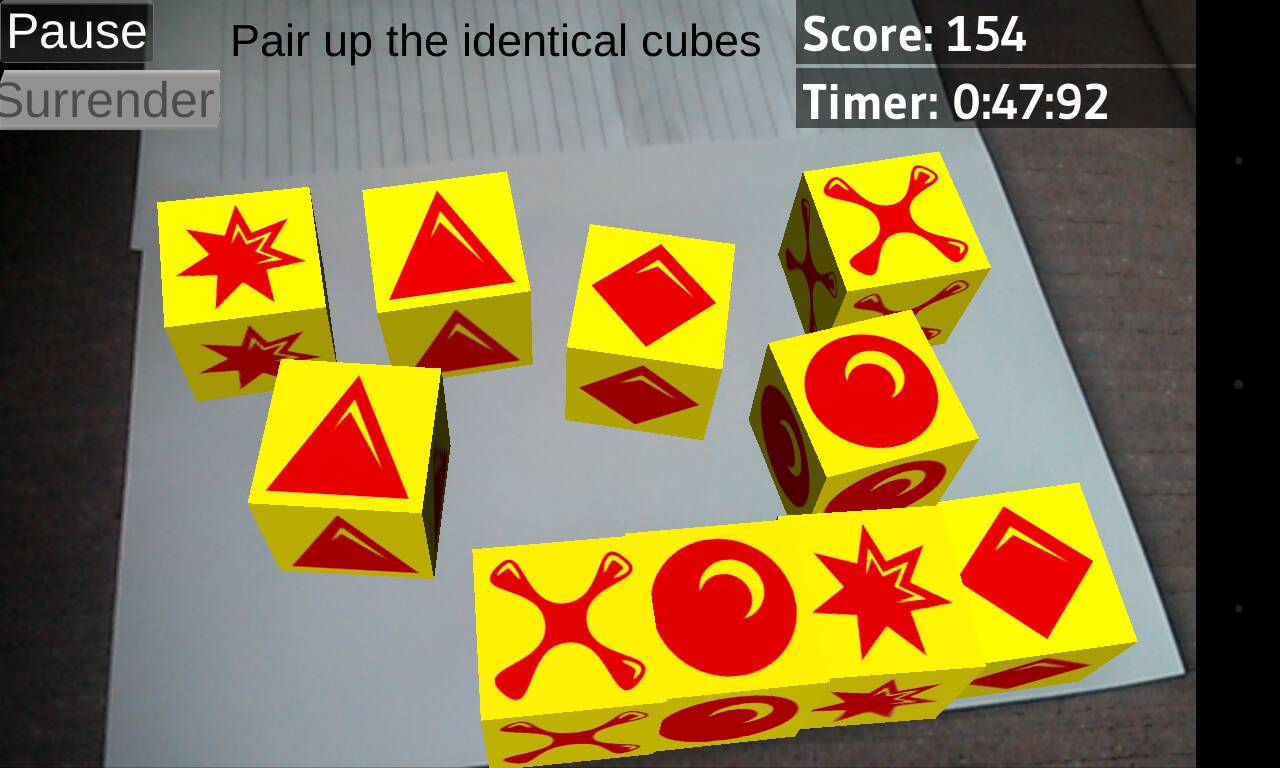
\includegraphics[width=0.9\textwidth]{images/match_cubes.jpg}
		\vspace{-10pt}
		\caption{Screenshot of a mini-game.}
		\label{fig:screenshot_mini-game}
	\end{minipage}
\end{figure}

\begin{figure}[ht]
	\capstart
	\centering
	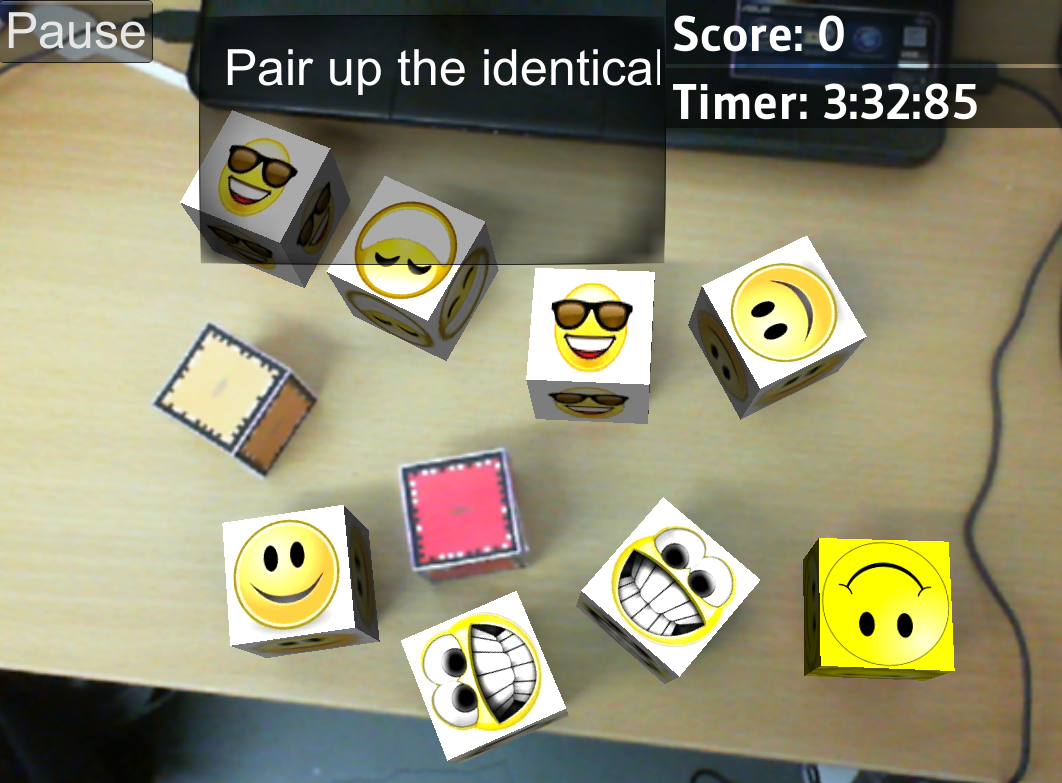
\includegraphics[width=0.8\textwidth]{images/MatchCubes}
	\caption{Match Cubes minigame}
	\label{fig:match_cubes}
\end{figure}

\paragraph{}
These two pcitures shows our current UI and what we had in the beginning.
Our first version used the default Unity style for both buttons and info boxes.
While it is funcitonal it is not very nice to look at and is too distracting in a enviroment such as this.
To rectify this we created our own UI styles to use instead of the default.
By removing as many distracting elements from the UI as possible we leave much more space open so the user can use more of the
screen to look for the cubes without having the UI be in the way.



\newpage
\subsection{Program flow chart}

\begin{figure}[ht]
	\capstart
	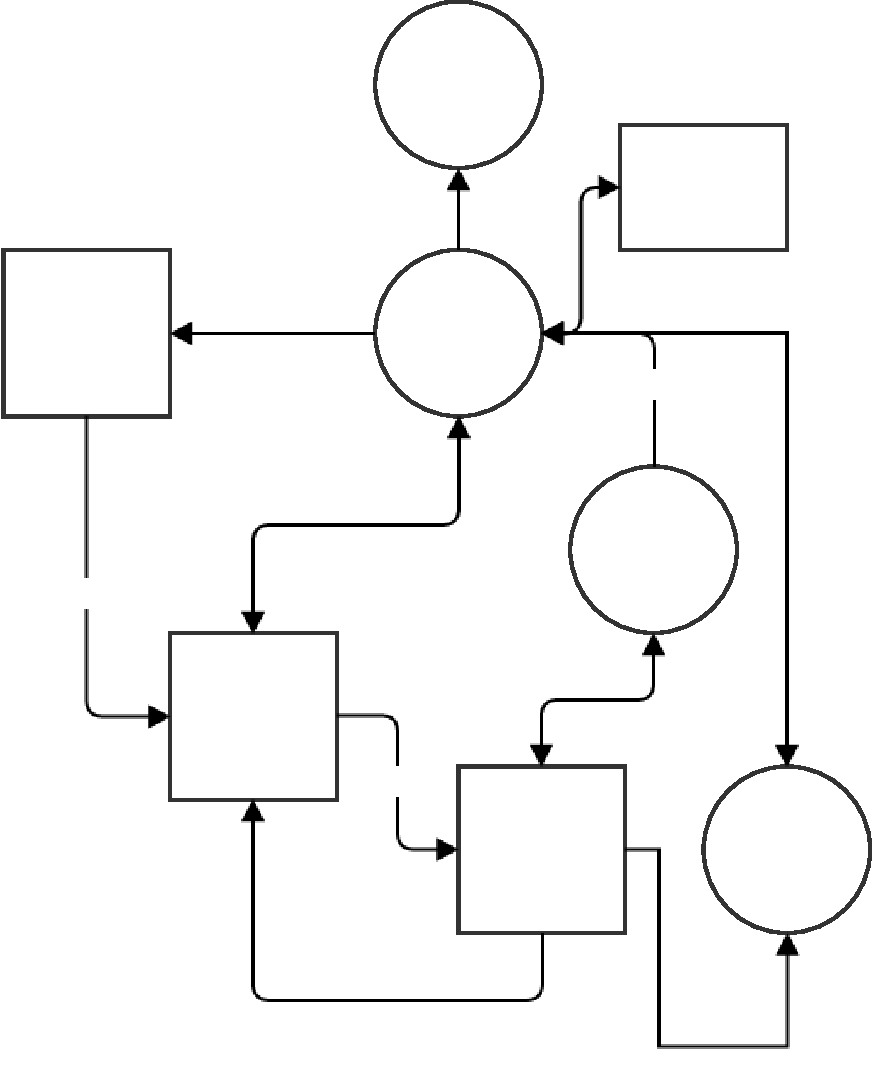
\includegraphics[width=\textwidth]{images/user_flow_chart}
	\caption[Program flow chart]{How a user maneuvers in the program.}
	\label{fig:program_flow_chart}
\end{figure}

Upon starting the program the user is presented with the main menu.
The main menu consists of four sets of buttons.

One set is the buttons that each lead to a single mini-game. 
When clicked they will take the player to the loading screen of the appropriate mini-game where the player can read instructions for the game and see current high-scores for that game.
After clicking the play button the user is taken into the game where the user can either play the mini-game or press the pause button.
If the user presses the pause button a pause screen is shown with the options of resuming the game, restarting from level one or go back to the main menu.

After the mini-game is completed the user is taken back to the loading screen if there is more levels left of the mini-game, otherwise the high-score list is shown.
The high-score lets the user go back to the main menu.

Back in the main menu, if the user presses the button "Change username" the user will be presented with a input field where a name can be entered, upon submitting a name the user will be brought back to the main menu.

If the user presses the "quit" button the application exits.

The last button on the main menu is the "Play all games" button. When the user presses this button it will play all the available mini-games in sequential order.